\documentclass[10pt,usepdftitle=false,aspectratio=169]{beamer}
% \documentclass[10pt,usepdftitle=false,aspectratio=169,handout]{beamer}

\usepackage{subfig}
\usepackage{graphicx}
\graphicspath{{../Figures/}}

\input{preamble_talk}
\usepackage{tcolorbox}
\usepackage{changepage}
\usepackage{arydshln}       %for dashed lines

% Assets included in preamble
\newcommand{\assetsDIR}{../Figures/assets}

% Add speaker notes to talk
% \setbeameroption{hide notes} % Only slides
%\setbeameroption{show only notes} % Only notes
% \setbeameroption{show notes on second screen}

\usetikzlibrary{external}
\usetikzlibrary{positioning}
\tikzset{main node/.style={circle,fill=white,draw,minimum size=1cm,inner sep=0pt},}
% \tikzexternalize[mode=list and make]
% use  make -j 4 -f talk.makefile to compile with 8 parallel threads (this is what it takes to max out the machine, depsite it having 4 cores)
\tikzset{external/force remake=false}
\tikzsetexternalprefix{external/}


%\setbeamersize{text margin left=0pt,text margin right=0pt} 
\begin{document}

\tikzexternaldisable

% %%%%%%%%%%%%%%%%%%%%%%%%%%%%%%%%%%%%%%%%%%%%%%%%%%%%%%%%%%%%%%%%%%%%%%%%%%%%%%%%%%%%%%%%%
% %                                     TITLE                                             %
% %%%%%%%%%%%%%%%%%%%%%%%%%%%%%%%%%%%%%%%%%%%%%%%%%%%%%%%%%%%%%%%%%%%%%%%%%%%%%%%%%%%%%%%%%

\section{Introduction}

\begin{frame}
  \title{{\bf Wasserstein t-SNE}\\[4mm]{}
  \vspace*{-.7cm}}
  \author{Fynn Bachmann \vspace{-1cm}} \date{July \nth{29}, 2021}

  \vspace{-1.5cm}
  \maketitle
  \vspace{-1.0cm}

  \begin{columns}
    \column{0.45\textwidth}
    \includegraphics[width=\textwidth]{\assetsDIR/UT_WBMW_Rot_RGB.pdf}\hfill
    % \column{.45\textwidth}
    \column{0.45\textwidth}
    \dre{Faculty of Science\\
    Department of Computer Science\\
    {\small Chair for the Methods of Machine Learning}}
    % \includegraphics[width=.8\textwidth]{\assetsDIR/MPI-IS-WortBildMarke.png}\\
    % \includegraphics[width=.8\textwidth]{\assetsDIR/imprs-is-logo.pdf}\\
    % \parbox[c]{.2\textwidth}{\centering\includegraphics[height=1.2cm]{\assetsDIR/ERC.png}}
    % \parbox{.75\textwidth}{\scriptsize \color{ERC_ora}some of the presented work is supported\newline by the European Research Council.}
  \end{columns}

  \thispagestyle{empty}
  \setcounter{framenumber}{0}

  %%%%%%%%%%%%%%%% ANIMATED LOGO %%%%%%%%%%%%%%%%
  % \tikzifexternalizing{}{%
  % \begin{tikzpicture}[remember picture,overlay]
  % \node[anchor=south,yshift=-5mm] at (current page.south)
  % {\animategraphics[width=0.9995\paperwidth,autoplay,loop]{36}{\assetsDIR/logo_TU_169_}{0}{39}};
  %   \end{tikzpicture}%
  % }%
  %%%%%%%%%%%%%% END OF ANIMATED LOGO %%%%%%%%%%%

  %%%%%%%%%%%%%%%% STATIC LOGO %%%%%%%%%%%%%%%%%%
  \tikzifexternalizing{}{%
  \begin{tikzpicture}[remember picture,overlay]
   \node[anchor=south,yshift=-5mm] at (current page.south)
  {\includegraphics[width=0.9995\paperwidth]{\assetsDIR/logo_TU_169_1.pdf}};
  \end{tikzpicture}%
  }%
  %%%%%%%%%%%%%% END OF STATIC LOGO %%%%%%%%%%%%%

\end{frame}
\tikzexternalenable

\setlength{\figurewidth}{\textwidth}
\setlength{\figureheight}{.9\textheight}

% %%%%%%%%%%%%%%%%%%%%%%%%%%%%%%%%%%%%%%%%%%%%%%%%%%%%%%%%%%%%%%%%%%%%%%%%%%%%%%%%%%%%%%%%%
% %                                     INTRO                                             %
% %%%%%%%%%%%%%%%%%%%%%%%%%%%%%%%%%%%%%%%%%%%%%%%%%%%%%%%%%%%%%%%%%%%%%%%%%%%%%%%%%%%%%%%%%

%%%%%%%%%%%%%%%%



\begin{frame}\frametitle{Master Thesis}\framesubtitle{Machine Learning}\titlemark{April - September 2021}
   \begin{block}{Topic Description}
   We want to develop a method to cluster/visualize a high dimensional dataset $\X$, that contains \textit{hierarchical structure}, i.e: where each datapoint $\X_i$ is a probability distribution from which we have an arbitrary amount of samples. These samples can be used to compute the mean, but also other moments of $\X_i$ such as covariance etc.
\end{block}
\begin{itemize}
\item Which datasets exist where each datapoint itself is a probability distribution? \item How are they visualized/clustered now, and which metrics on probability distributions can improve clustering? 
\end{itemize} 
   
\end{frame}




\section{Wasserstein Distance}

\begin{frame}{Hierarchical Data}\framesubtitle{German Federal Election 2017}
\LargeFigure{GER/Correlation_KielDresden ISPDAfD.pdf}
\end{frame}


\begin{frame}{Wasserstein Distance}
\begin{defi}
Let $\N_1, \N_2$ be two Gaussian distributions with $\N_i = (m_i, C_i)$. The 2-Wasserstein distance of these distributions is then given by:
$$W(\N_{1}, \N_{2})^{2} :=\left\|m_{1}-m_{2}\right\|_{2}^{2}+\text { trace }\left(C_{1}+C_{2}-2\left(C_{2}^{1 / 2} C_{1} C_{2}^{1 / 2}\right)^{1 / 2}\right)$$
\end{defi}

By introducing a hyperparameter $\lambda \in [0,1]$, we can put emphasis either on means or covariances.

\begin{block}{Convex Generalization:}
$$W(\N_{1}, \N_{2})^{2} := (1-\lambda) \cdot \left\|m_{1}-m_{2}\right\|_{2}^{2}+ \lambda \cdot  \text { trace }\left(C_{1}+C_{2}-2\left(C_{2}^{1 / 2} C_{1} C_{2}^{1 / 2}\right)^{1 / 2}\right)$$
\end{block}
\end{frame}


\begin{frame}{Proof of Concept}\framesubtitle{Hierarchical Gaussian Mixture}
\LargeFigure{HGM/CleanExample}
\end{frame}

\section{t-SNE Embeddings}

{
\usebackgroundtemplate{
  \tikz[overlay,remember picture] 
  \node[opacity=0.8, at=(current page.south east),anchor=south east,inner sep=0pt] {
    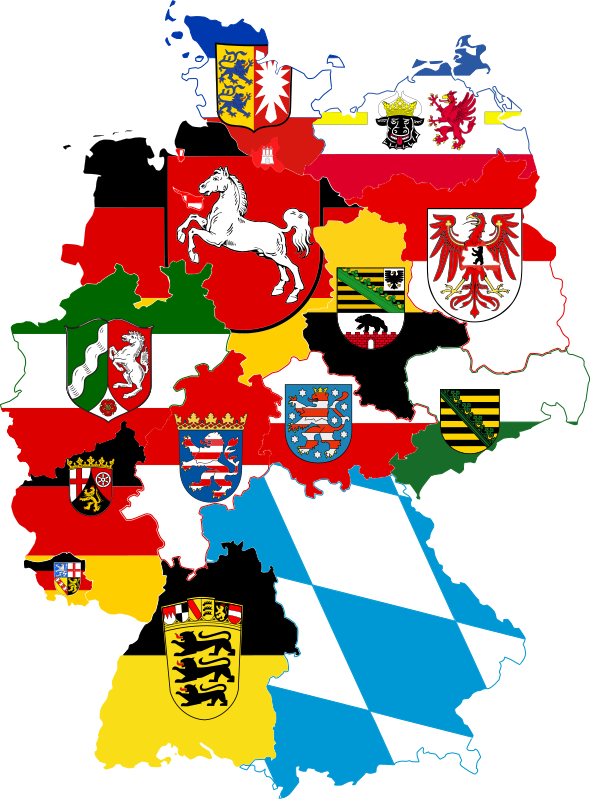
\includegraphics[height=0.9\textheight]{assets/Germany.png}};
}
\begin{frame}{Bundestagswahl 2017}\framesubtitle{German Election}\titlemark{Picture by Dimitri Averni, CC BY-SA 3.0}
 \begin{itemize}
    \item 88499 Wahlbezirke from 299 Wahlkreise 
    \item 6 features (voting results of major parties)
    \item 16 federal states as labels
\end{itemize}
\end{frame}
}

\begin{frame}{Wasserstein t-SNE Embedding}\framesubtitle{German Federal Election 2017}
\LargeFigure{GER/Embedding_small.pdf}
\end{frame}

\begin{frame}{Feature Analysis}
\framesubtitle{German Federal Election 2017}
\LargeFigure{GER/FeatureMeans.pdf}
\end{frame}

\begin{frame}{Correlation Analysis}
\framesubtitle{German Federal Election 2017}
\LargeFigure{GER/Correlation.pdf}
\end{frame}


\section{Exact Wasserstein}

{
\usebackgroundtemplate{
  \tikz[overlay,remember picture] 
  \node[opacity=0.8, at=(current page.south east),anchor=south east,inner sep=0pt] {
    \includegraphics[height=0.9\textheight]{assets/Europe.jpeg}};
}
\begin{frame}{European Values Study}\framesubtitle{Questionnaire}
\titlemark{Picture from \url{https://www.enisa.europa.eu/}}
 \begin{itemize}
    \item 37688 interviews from 114 European NUTS-1 regions
    \item 20 questions per interview with options from 1 and 10
    \item variety of different topics \\(i.e. environment, democracy, morality)
    \item 34 countries as labels
\end{itemize}
\end{frame}
}

\begin{frame}{Wasserstein t-SNE Embedding}\framesubtitle{European Values Study}
\LargeFigure{EVS/Embedding.pdf}
\end{frame}

\begin{frame}{Correlation Example}\framesubtitle{two features}
\LargeFigure{EVS/Correlation_plchv143v187.pdf}
\end{frame}

\begin{frame}{Exact Wasserstein Distance}\framesubtitle{one feature}
\LargeFigure{Wasserstein/Experiments1D.pdf}
\end{frame}

\begin{frame}{Exact Wasserstein Distance}\framesubtitle{scalable in samples}
{\begin{figure}
\includegraphics[height=0.9\figureheight,keepaspectratio]{Wasserstein/ExperimentsHistogram.pdf}
\end{figure}}
\end{frame}


\begin{frame}{Exact Wasserstein Distance}\framesubtitle{scalable in features}
\LargeFigure{Wasserstein/ExperimentsUniform.pdf}
\end{frame}


\begin{frame}{Exact Wasserstein t-SNE Embedding}\framesubtitle{European Values Study}
\LargeFigure{EVS/WassersteinComparison.pdf}
\end{frame}


\section{Outlook}

\begin{frame}{Outlook}\framesubtitle{for future work}
 \begin{itemize}
    \item Can we simplify the exact Wasserstein Distance Computation?
    \item Which other datasets exist, where this method improves visualization (e.g. medical data)?
\end{itemize}
\end{frame}


\end{document}

